\documentclass[11pt]{article}  
\usepackage[margin=1in]{geometry}
\parindent=0in
\parskip=8pt
\usepackage{fancyhdr,amssymb,amsmath, graphicx, listings,float,subfig,enumerate,epstopdf,color,multirow,setspace,bm,textcomp}
\usepackage[usenames,dvipsnames]{xcolor}
\usepackage{hyperref}
\usepackage{graphicx}
\graphicspath{{./Images}}

\pagestyle{fancy}


\begin{document} 

\lhead{Assignment \# 6}
\chead{Robert Denim Horton}
\rhead{\today}

\begin{center}\begin{Large}
CS 4720/5720 Design and Analysis of Algorithms

Homework \#6

Student: (Robert Denim Horton)
\end{Large}
\end{center}


\section*{Answers to homework problems:}

\begin{enumerate}
	% Question 1
	\item Say whether the following claim is true or false, and provide a brief (1-3 sentence) explanation for your answer. \\
	\begin{quote}
		 Claim: If player A in a two-person game has a dominant strategy $s_A$, then there is a pure strategy Nash equilibrium in which player A plays $s_A$ and player B plays a best response to $s_A$. 
	\end{quote}

	% Question 3
	\setcounter{enumi}{2}
	\item Find all pure strategy Nash equilibria in the game below. In the payoff matrix below the rows correspond to player A’s strategies and the columns correspond to player B’s strategies. The first entry in each box is player A’s payoff and the second entry is player B’s payoff.
	\begin{center}
		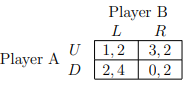
\includegraphics[scale=1.0]{Figure1.1}
	\end{center}
	% Question 4
	\item  Consider the two-player game with players, strategies and payoffs described in the following game matrix.
	\begin{center}
		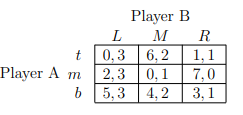
\includegraphics[scale=1.0]{Figure1.2}
	\end{center}
	\begin{enumerate}[(a)]
		% Question 4: Part 1
		\item Does either player have a dominant strategy? Explain briefly (1-3 sentences).
		% Question 4: Part 2
		\item Find all pure strategy Nash equilibria for this game.
	\end{enumerate}

	% Question 5
	\item Consider the following two-player game in which each player has three strategies.\\
	\begin{center}
		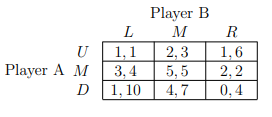
\includegraphics[scale=1.0]{Figure1.3}\\
	\end{center}
	Find all the (pure strategy) Nash equilibria for this game.\\
\end{enumerate}
\end{document}
